\documentclass[11pt]{article}


\renewcommand{\textfraction}{0.001}
\renewcommand{\topfraction}{0.999}   
\renewcommand{\bottomfraction}{0.999}


\usepackage[T1]{fontenc}
\usepackage[utf8]{inputenc}
\usepackage[english]{babel}
\usepackage{mathptmx}
\usepackage{a4}
\usepackage{makeidx}
\makeindex
\usepackage{ulem}
\usepackage{graphicx}
\usepackage{tikz}
\usepackage[slc=on]{caption} %für subfloats
\usepackage{subcaption}
\usepackage{amsmath}
\usepackage{amssymb}
\usepackage{amscd}
\usepackage[numbers,square,sort&compress]{natbib}
\usepackage{fancyhdr}
\usepackage{multirow}
\usepackage{enumitem}
\setlist{nosep}
\renewcommand{\labelitemi}{--}

\usepackage{url, hyperref}


\usepackage{listings}
\usepackage{color}

\definecolor{mygreen}{rgb}{0,0.6,0}
\definecolor{mygray}{rgb}{0.9,0.9,0.9}
\definecolor{mymauve}{rgb}{0.58,0,0.82}

\lstset{ %
  backgroundcolor=\color{mygray},   % choose the background color; you must add \usepackage{color} or \usepackage{xcolor}
  basicstyle=\footnotesize\ttfamily,        % the size of the fonts that are used for the code
  breakatwhitespace=false,         % sets if automatic breaks should only happen at whitespace
  breaklines=true,                 % sets automatic line breaking
  captionpos=b,                    % sets the caption-position to bottom
  commentstyle=\color{mygreen},    % comment style
  deletekeywords={...},            % if you want to delete keywords from the given language
  escapeinside={\%*}{*)},          % if you want to add LaTeX within your code
  extendedchars=true,              % lets you use non-ASCII characters; for 8-bits encodings only, does not work with UTF-8
  frame=none,                    % adds a frame around the code
  keepspaces=true,                 % keeps spaces in text, useful for keeping indentation of code (possibly needs columns=flexible)
  keywordstyle=\color{red},       % keyword style
  language=,                 % the language of the code
  morekeywords={begin, end, documentclass,usepackage,author, maketitle, newpage, title, date, linespread, selectfont, section, subsection, subsubsection, paragraph, subparagraph, tableofcontents, item, verb, setlength, parindent, parskip, cite, parencite, footcite, makeindex, printindex, includegraphics, textwidth, textbf, cline, multirow, multicolumn, hline, footnote,blindtext,renewcommand, pagestyle, label, ref, nameref, pageref, makebox, fbox, framebox, mbox, raggedleft, raggedright, centering, textrm, textsl, textit, textsc, textsf, texttt, setcounter},            % if you want to add more keywords to the set
  numbers=left,                    % where to put the line-numbers; possible values are (none, left, right)
  numbersep=5pt,                   % how far the line-numbers are from the code
  numberstyle=\tiny\color{mygray}, % the style that is used for the line-numbers
  rulecolor=\color{black},         % if not set, the frame-color may be changed on line-breaks within not-black text (e.g. comments (green here))
  showspaces=false,                % show spaces everywhere adding particular underscores; it overrides 'showstringspaces'
  showstringspaces=false,          % underline spaces within strings only
  showtabs=false,                  % show tabs within strings adding particular underscores
  stepnumber=2,                    % the step between two line-numbers. If it's 1, each line will be numbered
  stringstyle=\color{mymauve},     % string literal style
  tabsize=2,                       % sets default tabsize to 2 spaces
  title=\lstname                   % show the filename of files included with \lstinputlisting; also try caption instead of title
}         % Palatino needs more leading (space between lines)

\lstset{
  literate={ö}{{\"o}}1
           {ä}{{\"a}}1
           {ü}{{\"u}}1
           {Ü}{{\"U}}1
}
\usepackage[T1]{fontenc}

%
%
%%
%
%
\definecolor{red}{rgb}{1,0,0}
\definecolor{green}{rgb}{0,1,0}
\definecolor{blue}{rgb}{0,0,1}
\definecolor{darkblue}{rgb}{0,0,0.8}

\definecolor{yellow}{rgb}{1,1,0}
\definecolor{lightblue}{rgb}{0,1,1}
\definecolor{magenta}{rgb}{1,0,1}
\definecolor{lightgrey}{rgb}{0.5,0.5,0.5}
\definecolor{grey}{rgb}{0.35,0.35,0.35}
\definecolor{darkgrey}{rgb}{0.2,0.2,0.2}
\definecolor{ockerrot}{rgb}{0.859,0.375,0.152}




\pagestyle{headings}
%

%\fancyfoot[RO]{\textsf{\nouppercase{\leftmark}}}
\cfoot{~}

\fancypagestyle{plain}{\fancyhf{}}




\setlength{\parskip}{1.5ex plus 0.5ex minus 0.2ex}
\setlength{\parindent}{0pt}

\begin{document}
\begin{titlepage}
\hspace*{\fill}
\includegraphics[width=0.4\textwidth]{uzh_logo_e_pos}\vspace{2cm}\hspace*{\fill}

\centering
\LARGE {Eine kleine \LaTeX{} Zusammenfassung} \\[1cm]
\normalsize{Philipp Gloor\\Informatikdienste der Universit"at Z"urich\footnote{philipp.gloor@uzh.ch}} 
\end{titlepage}
\newpage
{\setlength{\parskip}{0pt}
\tableofcontents
}
\newpage

\section*{Preface}

This document serves as a small compendium for working with \LaTeX. It is anything but complete but it should help to get you started in case you forgot some things. If you want to know more about a certain package it is always worth it to read the package documentation. If your \LaTeX\ folder is in your path environment you can use \texttt{texdoc} \textit{packagename} to open the documentation for said manual. Another good place to start is the \LaTeX\ wikibook \url{https://en.wikibooks.org/wiki/LaTeX}.

If you have a specific problem and you do not know how to proceed you can first try google and if this does not help you can visit \url{tex.stackexchange.com} and try to ask your question there.

\section[Hello World - ein erstes Beispiel]{Hello World}
\begin{lstlisting}
\documentclass[10pt]{article}
\usepackage[T1]{fontenc} %Kommentar
\usepackage[utf8]{inputenc}
\begin{document}
Hello World
\end{document}
\end{lstlisting}

\begin{itemize}
\item \verb+\documentclass[10pt]{article}+ defines the document class (article, report, book). 10pt is the base font size for the document.
\item \verb+\usepackage[•]{•}+ laods the respective package.
\item \verb+\begin{document} \end{document}+ The begin and end of the content of the document
\item \% used for comments.
\end{itemize}

Code written \textbf{before} \verb+\begin{document}+ is called preamble. Every command that is not content belongs there (\textit{usepackage} commands e.g.)

\newpage

\section{Title page}
\begin{lstlisting}
\documentclass[10pt]{article}

\usepackage[T1]{fontenc}
\usepackage[utf8]{inputenc}

\usepackage[english]{babel}


\title{\LaTeX\ leicht gemacht}

\author{Hans Muster\\Universität Hier\thanks{bla@gmail.com} \and Peter Lustig\\Universität Dort\thanks{blub@gmail.com}}
\date{\today}
\begin{document}

\maketitle

\newpage


\end{document}
\end{lstlisting}

\begin{itemize}
\item \verb+\usepackage[english]{babel}+ is the language package for \LaTeX. Responsible for proper hyphenation.
\item \verb+\title{•}+ defines the title. This command does not create the title page. For this you need \verb+\maketitle+ (which will then use the information provided by \verb+\title{}+.
\item \verb+\author{•}+ defines one or more authors if connected with an \verb+\and+.
\item \verb+\\+ inserts new line
\item \verb+\date{\today}+ inserts current date to the title page. \verb+\today+ can be replaced with any string, does not necessarily have to be a date.
\item \verb+\maketitle+ Places the title page where the command is writting. Usually just after \verb+\begin{document}+.
\item \verb+\newpage+ inserts new page.
\end{itemize}

Alternativ kann man seine Titelseite auch selber gestalten. Dafür bietet sich die \texttt{titlepage}-Umgebung an. Also

\begin{lstlisting}
\begin{titlepage}

% hier kommmt alles, was auf die Titelseite kommen soll.

\end{titlepage}
\end{lstlisting}



\section{Anf"uhrungszeichen}
\begin{lstlisting}
\documentclass[10pt, a4paper]{article}
\usepackage[T1]{fontenc} 
\usepackage[utf8]{inputenc}
\usepackage[english]{babel}

\setlength{\parindent}{0pt}
\begin{document}
``Test''  - englische Form\\
"`Test"'  - deutsche Form\\
"<Test"> - franz"osische Form
\end{document}
\end{lstlisting}

Um Anf"uhrungs- und Schlusszeichen richtig zu setzen, braucht man spezielle Befehle (Wenn man es aber nicht so genau nehmen will, reichen auch die "normalen"{} Anf"uhrungszeichen.
\begin{itemize}
\item Englische Form: 2 Grave-Akzente setzen das Anf"uhrungszeichen, 2 Apostroph-Zeichen f"ur das Abf"uhrungszeichen.
\end{itemize}



\section{Zeilenabstand}

\begin{lstlisting}
\usepackage{blindtext}

\begin{document}
\linespread{2}\selectfont
\blindtext

\end{document}
\end{lstlisting}

\begin{itemize}
\item \verb+\linespread{x}+ Multipliziert den Standardzeilenabstand (=1) mit dem Faktor $x$. Also macht \verb+\linespread{2}+ einen doppelten Zeilenabstand.
\item \verb+\selectfont+ muss angeh"angt werden, um den neuen Zeilenabstand zu aktivieren.
\end{itemize}


\newpage

\section{Gliederungen}
\begin{lstlisting}
\documentclass[10pt]{article}
\usepackage[T1]{fontenc}
\usepackage[utf8]{inputenc}

\usepackage[english]{babel}

%\setcounter{secnumdepth}{5}
%\setcounter{tocdepth}{5}


\begin{document}
\tableofcontents

\newpage

\section{Einleitung}
Hier steht dann der Text der zur Einleitung gehört. Die Nummerierung geschieht automatisch, genau so wie die Formatierung. Und so weiter und so fort.

\subsection{Vertiefung der Einleitung}
Das hier ist dann eine Untersektion von Einleitung.

\subsubsection{Noch eine stufe tiefer (so wie Inception)}
Die subsubsection ist die letzte nummerierte Struktur in einem Standard \LaTeX\  Dokument.

\paragraph{Paragraph}
Paragraphen sind die zweitletzte Stufe der Gliederung. Sie werden normalerweise nicht nummeriert.

\subparagraph{Subparagraph}
Subparagraph ist die letzte Stufe. Sie werden wie die Paragraphen nicht nummeriert.

\end{document}
\end{lstlisting}

\begin{itemize}
\item \verb+\tableofcontents+ erstellt an dieser Stelle ein Inhaltsverzeichnis, basierend auf den Gliederungsbefehlen, die sich im Dokument befinden.
\item \verb+\section{•}+ erstellt einen Sektionstitel an dieser Stelle. Der Platzhalter innerhalb der Klammern muss mit dem Titel der Sektion ausgef"ullt werden. Der Name der Sektion und deren Nummer taucht dann auch im Inhaltsverzeichnis auf.
\item Gleiches gilt f"ur weitere Gliederungsstufen wie zum Beispiel \verb+\subsection{•}+, welche eine Stufe unter \verb+\section{•}+ steht.
\item Die beiden \texttt{setcounter}-Befehle in Zeile 7 und 8 definieren wie tief Gliederungsstufen nummeriert werden (\texttt{secnumdepth}) und im Inhaltsverzeichnis auftauchen (\texttt{tocdepth}). 3 ist die Standardtiefe, das heisst, \texttt{subsubsection} ist die letzte Gliederungsstufe die nummeriert wird und im Inhaltsverzeichnis erscheint. Stufe 4 gilt dann f"ur \texttt{paragraph} und Stufe 5 f"ur \texttt{subparagraph}.
\end{itemize}

\newpage 
\section{Auflistungen}

\begin{lstlisting}
\documentclass[10pt]{article}
\usepackage[T1]{fontenc}
\usepackage[utf8]{inputenc}
\usepackage{enumitem}
\usepackage[english]{babel}

\usepackage{pifont}

\begin{document}

\begin{itemize}
\item Erstes Item
\item[\ding{43}] Zweites Item
\end{itemize}

\begin{enumerate}
\item Erster Punkt
\item Zweiter Punkt
\end{enumerate}

\end{document}
\end{lstlisting}

\begin{itemize}
\item \verb+\usepackage{pifont}+ ist ein Paket, das gebraucht wird um gewisse Sonderzeichen darzustellen. Dieses Paket hat keine optionalen Parameter beim Aufruf ([] enthalten optionale Argumente).
\item \verb+\begin{itemize} \end{itemize}+ er"offnet eine unnummerierte Auflistung.
\item \verb+\item+ ist der Befehl, der einen neuen Aufz"ahlungspunkt einf"ugt. Jeglicher Text der darauf folgt, geh"ort zu diesem Punkt.
\item \verb+\item[•]+ Man kann auch eigene Aufz"ahlungszeichen definieren innerhalb der eckigen Klammern, direkt nach \verb+\item+.
\item \verb+\begin{enumerate} \end{enumerate}+ er"offnet eine nummerierte Auflistung
\item Das \verb+enumitem+ Paket ermöglicht viele Anpassungsmöglichkeiten. Siehe dazu die Dokumentation: \url{http://mirrors.ctan.org/macros/latex/contrib/enumitem/enumitem.pdf}
\end{itemize}

Aufz"ahlungen k"onnen auch ineinander verschachtelt werden. F"ur eine Liste mit allen m"oglichen Sonderzeichen, die man in \LaTeX{} verwenden kann ist hier ein Dokument, welches diese auflistet.
\url{http://www.tex.ac.uk/tex-archive/info/symbols/comprehensive/symbols-a4.pdf}
\newpage
\section{Schriftarten und Schriftschnitte}

\begin{lstlisting}
\documentclass[10pt, a4paper]{article}
\usepackage[T1]{fontenc}
\usepackage[utf8]{inputenc}

\usepackage[english]{babel}

\usepackage{blindtext}

%\usepackage[sfdefault]{quattrocento} %Für eine andere Schriftart
%\usepackage[T1]{fontenc} %Gehört zum Befehl um die Schriftart zu wechseln



\begin{document}

\section{Schriften in \LaTeX}

\subsection{Überschaubare Textbereiche}

\textrm{Schrift mit Serifen} \\
\textbf{Fette Schrift}\\
\textsf{Serifenlose Schrift}\\
\textit{Kursive Schrift}\\
\textsl{Geneigte Schrift}\\
\texttt{Typewriter}\\
\textsc{Kapitälchen (small caps)}

\subsection{Längere Textpassagen}

{\ttfamily \blindtext}

{\sffamily \blindtext}

{\bfseries \blindtext}

{\itshape \blindtext}

{\slshape \blindtext}

{\scshape \blindtext}
\end{document}
\end{lstlisting}
\renewcommand{\arraystretch}{1.2}
\begin{table}[b]
\center
\begin{tabular}{|c|c|c|}
\hline 
Befehl 1 & Befehl 2 & Schriftschnitt \\ 
\hline 
\verb+\textrm{•}+ & \verb+\rmfamily+ & Roman \\ 
\hline 
\verb+\textbf{•}+ & \verb+\bfseries+ & \textbf{Fett} \\ 
\hline 
\verb+\textsf{•}+ & \verb+\sffamily+ & \textsf{Serifenlos} \\ 
\hline 
\verb+\textit{•}+ & \verb+\itshape+ & \textit{Italic} \\ 
\hline 
\verb+\textsl{•}+ & \verb+\slshape+ & \textsl{Geneigt} \\ 
\hline 
\verb+\texttt{•}+ & \verb+\ttfamily+ & \texttt{Typewriter} \\ 
\hline 
\verb+\textsc{•}+ & \verb+\scshape+ & \textsc{Small Caps} \\ 
\hline 
\end{tabular} 
\caption{Schriftbefehls"ubersicht}
\end{table}

\begin{itemize}
\item \verb+\usepackage{blindtext}+ erlaubt das Setzen von Blindtext, so dass man schnellt sieht - ob ein Layoutbefehl richtig wirkt.
\item \verb+\usepackage[sfdefault]{quattrocento}+ "andert die Schriftart. Generell w"urde ich vom "Andern der Schriftart abraten. Unter \url{http://www.tug.dk/FontCatalogue/} findet man die Befehle, die man f"ur diverse Schriftarten braucht. Man sollte beachten, dass die Schriftart unter Umst"anden auf dem Computer nicht installiert ist und der Befehl dann nicht funktioniert.
\end{itemize}

\newpage

\section{Schriftgr"ossen}

\begin{lstlisting}
\documentclass[10pt, a4paper, draft]{article}
\usepackage[T1]{fontenc}
\usepackage[utf8]{inputenc}

\usepackage[english]{babel}
\usepackage{blindtext}

\begin{document}

\section{Schriftgrössen in \LaTeX}

\subsection{tiny}
{\tiny \blindtext\par}

\subsection{scriptsize}
{\scriptsize \blindtext\par}

\subsection{footnotesize}
{\footnotesize \blindtext\par}

\subsection{small}
{\small \blindtext\par}

\subsection{normalsize}
{\normalsize \blindtext\par}

\subsection{large}
{\large \blindtext\par}

\subsection{Large}
{\Large \blindtext\par}

\subsection{LARGE}
{\LARGE \blindtext\par}

\subsection{huge}
{\huge \blindtext\par}

\subsection{Huge}
{\Huge \blindtext\par}

\end{document}
\end{lstlisting}

\begin{itemize}
\item Die \{ \}-Klammern um die ganzen Befehle dienen hier als Gruppenklammern. Etwaige "Anderungen im Layout gelten nur innerhalb der Gruppenklammern.
\item Die Schriftgr"ossen sind relativ zur Basisschriftgr"osse des Dokumentes (definiert im ersten Befehl \verb+\documentclass[•]{•}+).
\item Die Option \texttt{draft} blendet Bilder im Dokument aus und zeigt an, wo Texte die Textbreite "uberschreiten (Meldung in Texmaker ist \textit{Overfull \textbackslash hbox})
\end{itemize}

\section{Verbose-Befehl}

Will man einen \LaTeX-Befehl explizit in einem Dokument verwenden, wie ich es in dieser Anleitung oft gemacht habe, braucht es einen speziellen Befehl. Denn wie soll \LaTeX\ wissen, dass der Befehl \textit{nicht} interpretiert werden soll?
Der Befehl ist der Verbose-Befehl und wird wie folgt angewendet.

\begin{lstlisting}
\verb+\dag+
\end{lstlisting}

Schreibe ich dieses Konstrukt in ein \LaTeX\-Dokument erhalte ich anstelle von \dag\ ein \verb+\dag+. Wichtig ist zu bemerken, dass die beiden Pluszeichen die \glqq Klammern\grqq dieses Befehls sind.

\section{Trennstriche und Silbentrennung}
\begin{lstlisting}
- %Trennstrich
-- %Gedankenstrich
--- %Doppelter Gedankenstrich
\end{lstlisting}

Falls die Worttrennung in \LaTeX\ fehlerhaft ist, kann man mit folgenden Befehlen nachhelfen

\begin{itemize}
\item \verb+\-+ in diesem Fall wird das Wort nur an den so gekennzeichneten Stellen getrennt. Trennstellen, die sich aus dem Trennalgorithmus ergeben, werden ignoriert. Beispiel: \verb+Uni\-ver\-si\-täts\-ver\-wal\-tung+
\item \verb+"-+ stellt eine zus"atzliche Trennstelle zu denen aus dem Trennalgorithmus zur Verf"ugung.
\item \verb+""+ definiert einen potentiellen Zeilenwechsel, wobei kein zus"atzlicher Trennstrich eingef"ugt wird. \verb+Di-""Methyl-""Aceton+
\end{itemize}

\section{Absatzabstand und -einzug}

\begin{lstlisting}
\setlength{\parindent}{0pt}
\setlength{\parskip}{1.5ex plus 0.5ex minus 0.2ex}
\end{lstlisting}

\begin{itemize}
\item \verb+\setlength{•}{•}+ ist der Befehl mit dem man definierte Dimensionsvariablen ver"andern kann.
\item \verb+\parskip+ ist die Variable, die den Abstand zwischen 2 Abs"atzen definiert. %\the\parskip \the\parindent
\item \verb+\parindent+ ist die Variable, die den Einzug in der ersten Zeile eines neuen Absatzes definiert.
\item Mithilfe von \texttt{plus} und \texttt{minus} kann man die Variable dynamisch gestalten und so \LaTeX\ gewissen Spielraum bei dem Seitenumbruch erm"oglichen.
\end{itemize}

\section{Zeilenumbruch}

\begin{lstlisting}
Franz jagt im komplett verwahrlosten Taxi quer durch Bayern\\
Franz jagt im komplett verwahrlosten Taxi quer durch Bayern\\[3cm]
Franz jagt im komplett verwahrlosten Taxi quer durch Bayern\\
\end{lstlisting}

Ergebnis:\\
Franz jagt im komplett verwahrlosten Taxi quer durch Bayern\\
Franz jagt im komplett verwahrlosten Taxi quer durch Bayern\\[1cm]
Franz jagt im komplett verwahrlosten Taxi quer durch Bayern\\

\begin{itemize}
\item \texttt{mm}: Millimeter
\item \texttt{cm}: Zentimeter
\item \texttt{in}: Inch (1 Inch = 2.54 cm)
\item \texttt{pt}: Punkt (1 Punkt $\approx \frac{1}{72} \text{in} \approx \frac{1}{3} \text{mm}$)
\item \texttt{em}: Breite des Buchstabens \texttt{M}; proportional zum Zeichensatz
\item \texttt{ex}: Breite des Buchstabens \texttt{x}; proportional zum Zeichensatz
\end{itemize}

\section{Absatzausrichtung}

\begin{lstlisting}
{ \raggedright %für linksbündig
Der Abstand zwischen den Absätzen soll 1.5ex betragen, der um maximal 0.5ex aufgeweitet und um höchsten 0.2ex gestaucht werden kann. Dieser und der folgende Absatz sollen linksbündig ausgerichtet werden. \par }

{ \raggedleft %für rechtsbündig
Der Abstand zwischen den Absätzen soll 1.5ex betragen, der um maximal 0.5ex aufgeweitet und um höchsten 0.2ex gestaucht werden kann. Dieser und der folgende Absatz sollen linksbündig ausgerichtet werden. \par }

{ \centering %zentriet
Der Abstand zwischen den Absätzen soll 1.5ex betragen, der um maximal 0.5ex aufgeweitet und um höchsten 0.2ex gestaucht werden kann. Dieser und der folgende Absatz sollen linksbündig ausgerichtet werden. \par}
\end{lstlisting}

{ \raggedright %für linksbündig
Der Abstand zwischen den Absätzen soll 1.5ex betragen, der um maximal 0.5ex aufgeweitet und um höchsten 0.2ex gestaucht werden kann. Dieser und der folgende Absatz sollen linksbündig ausgerichtet werden. \par }

{ \raggedleft %für rechtsbündig
Der Abstand zwischen den Absätzen soll 1.5ex betragen, der um maximal 0.5ex aufgeweitet und um höchsten 0.2ex gestaucht werden kann. Dieser und der folgende Absatz sollen linksbündig ausgerichtet werden. \par }

{ \centering %zentriet
Der Abstand zwischen den Absätzen soll 1.5ex betragen, der um maximal 0.5ex aufgeweitet und um höchsten 0.2ex gestaucht werden kann. Dieser und der folgende Absatz sollen linksbündig ausgerichtet werden. \par}

Der Abstand zwischen den Absätzen soll 1.5ex betragen, der um maximal 0.5ex aufgeweitet und um höchsten 0.2ex gestaucht werden kann. Dieser und der folgende Absatz sollen linksbündig ausgerichtet werden.

\section{Boxen}

\begin{lstlisting}
\mbox{Schifffahrtsgesellschaft}
\makebox[Breite][Ausrichtung]{Schifffahrtsgesellschaft}
\fbox{Schifffahrtsgesellschaft}
\framebox[Breite][Ausrichtung]{Schifffahrtsgesellschaft}
\end{lstlisting}

\mbox{Schifffahrtsgesellschaft}\\
\makebox[3cm][r]{Schifffahrtsgesellschaft}\\
\fbox{Schifffahrtsgesellschaft}\\
\framebox[3cm][l]{Schifffahrtsgesellschaft}

\begin{itemize}
\item Der Parameter \textit{Breite} muss zum Beispiel in \texttt{cm} angegeben werden.
\item F"ur die Ausrichtung hat man folgende Angaben zur Auswahl: \texttt{l, r, c, s}. Sie stehen f"ur \textit{left}, \textit{right}, \textit{center}, \textit{spread} (Blocksatz).
\end{itemize}

\newpage
\section{Referenzen}

\begin{lstlisting}
\documentclass[10pt]{article}
\usepackage[T1]{fontenc}
\usepackage[utf8]{inputenc}

\usepackage[english]{babel}

\usepackage{hyperref} %damit \nameref{} funktioniert

\begin{document}

\section{Einleitung \label{sec:Einleitung}}

Lorem ipsum dolor sit amet, consectetur adipiscing elit. Vivamus quis ligula et diam congue posuere quis vitae dolor. In hac habitasse platea dictumst. Sed pellentesque commodo justo sed interdum. Nullam malesuada, sem sit amet lobortis molestie, est eros lobortis felis, at interdum odio tellus auctor nisi. Pellentesque at libero risus, quis interdum massa. 
\newpage

\section{Theorie \label{sec:Theorie}}
Wie in der Sektion \ref{sec:Einleitung}: \nameref{sec:Einleitung} auf Seite \pageref{sec:Einleitung} gesehen.


\end{document}
\end{lstlisting}

\begin{itemize}
\item Das Paket \texttt{hyperref} braucht es nur, dass man sich auch auf den Namen einer Referenz (\verb+\nameref{}+) beziehen kann.
\item \verb+\label{labelname}+ setzt eine Referenz. Auf diese Referenz kann dann mit den anderen Befehlen darauf referenziert werden.
\item \verb+\ref{labelname}+ ruft die Referenz auf. Geh"ort das Label zu einer Sektion, f"ugt dieser Befehl die Nummer dieser Sektion ein.
\item \verb+\nameref{labelname}+ ruft den Namen der Referenz auf. Bei einer Sektion steht dann der Sektionsname im Text.
\item \verb+\pageref{labelname}+ ruft die Seitennummer der Referenz auf.
\end{itemize}

F"ur das Label kann ein beliebiger Name gew"ahlt werden. Es empfiehlt sich aber, ein gewisses Muster bei der Vergabe von Labelnamen anzuwenden:

\begin{itemize}
\item chap: chapter
\item sec:  section
\item subsec: subsection
\item fig:  figure
\item tab:  table
\item eq: equation
\item lst:  code listing
\item itm:  enumerated list item
\item app:  appendix subsection
\end{itemize}

\newpage

\section{Seitenlayout}
\begin{lstlisting}
\documentclass[10pt]{article}
\usepackage[T1]{fontenc}
\usepackage[utf8]{inputenc}

\usepackage[english]{babel}
\usepackage{blindtext}

\pagestyle{headings} %Andere optionen: plain, empty, headings

%http://en.wikibooks.org/wiki/LaTeX/Page_Layout#Customizing_with_fancyhdr

\usepackage{fancyhdr}

\setlength{\headheight}{15.2pt}

\pagestyle{fancy}


\renewcommand{\headrulewidth}{0.5pt} %Setzt die Breite der Kopfzeilenlinie auf 0.5pt
\renewcommand{\footrulewidth}{0.5pt} %Setzt die Breite der Fusszeilenlinie auf 0.5pt

\lhead{Übungsdokument} %Linker Teil vom Header
\chead{}               %Mittlerer Teil vom Header
\rhead{\leftmark} %Rechter Teil vom Header


\rfoot{\thepage}
\cfoot{}
\lfoot{}
\begin{document}



\section{Einleitung}
\blindtext

\newpage

\section{Theorie}
\blindtext


\end{document}
\end{lstlisting}

Im Standard kommen 3 verschiedene Seitenlayouts mit \LaTeX. \texttt{Empty}, \texttt{plain}, \texttt{headings} wobei bei der ersten Option keine Kopf- und Fusszeile erscheint. Bei \texttt{plain} hat man eine Seitennummer in der Fusszeile und bei \texttt{headings} kriegt man einen lebenden Kopfzeilentitel plus Seitenzahlen.

Falls man mit diesen Optionen unzufrieden ist, gibt es das Paket \texttt{fancyhdr}. Dort kann man mit gezielten Befehlen einzelne Kopf- und Fusszeilenabschnitte (left, center, right) steuern.

\section{Zitate}

\begin{lstlisting}
\documentclass[10pt, a4paper]{article}
\usepackage[T1]{fontenc} 
\usepackage[utf8]{inputenc}
\usepackage[english]{babel}

\usepackage{blindtext}

\begin{document}

\section{Quote-Umgebung}

\blindtext
\begin{quote}
\blindtext

\blindtext
\end{quote}

\newpage

\begin{quotation}
\blindtext

\blindtext
\end{quotation}
\blindtext
\end{document}
\end{lstlisting}

Will man einen Textteil zitieren, bieten sich zwei Umgebungen an.

\begin{itemize}
\item \verb+quote+ 'Deutsche' Version des Zitats. Kein Einzug bei neuem Absatz mit kleinem zus"atzlichem Abstand zwischen Abs"atzen.
\item \verb+quotation+ 'Englische' Version des Zitats. Einzug bei neuem Absatz ohne zusa"tzlichen Abstand zwischen Abs"atzen.
\end{itemize}

\newpage
\section{Fussnoten}

\begin{lstlisting}
\documentclass[10pt]{article}
\usepackage[T1]{fontenc}
\usepackage[utf8]{intputenc}

\begin{document}
Das ist die Einführung in einem Dokument und ich füge hier eine Fussnote hinzu\footnote{Das ist jetzt der Text, der in der Fussnote auftaucht}
\end{document}

\end{lstlisting}

Das ist die Einführung in einem Dokument und ich füge hier eine Fussnote hinzu\footnote{Das ist jetzt der Text, der in der Fussnote auftaucht}
\newpage

\section{Tabellen}

\begin{lstlisting}
\begin{tabular}[c]{c|c}
\hline
1 & 2 \\
\hline 
3 & 4\\
\hline
\end{tabular}
\end{lstlisting}
\begin{tabular}[c]{c|c}
\hline
1 & 2 \\
\hline 
3 & 4\\
\hline
\end{tabular}

Einfachstes Beispiel einer Tabelle. Diese Tabelle wird direkt im Fliesstext eingebunden und ist nicht freistehend (siehe sp"ater mit Gleitumgebungen - Floats).

\begin{itemize}
\item \verb+\begin{tabular}[c]{c|c}+ tabular erstellt eine Tabelle. Das optionale Argument \verb+[c]+ richtet die Tabelle zentriert am Text aus (weitere Optionen sind \texttt{t} (top) \texttt{b} (bottom).
\item \verb+{c|c}+ Die Tabelle besteht aus 2 Spalten (beide zentriert ausgerichtet - c steht f"ur center). Zwischen den beiden Spalten gibt es eine vertikale Trennlinie.
\item \verb+&+ ist das Tabulatorzeichen, zwischen den Zellen steht jeweils ein Tabulatorzeichen. Am Anfang und Endeeiner Zeile braucht es kein Tabulatorzeichen.
\item Die Zeile kann mit einen \verb+\\+ abgeschlossen werden.
\item \verb+\hline+ zeichnet eine horizontale Linie zwischen den Zeilen.
\item Die Anzahl Spalten wird via Befehl vorgegeben (\verb+{cccccc}+ definiert zum Beispiel 6 Spalten, alle zentriert ausgerichtet, \verb+{ll|rrcccc|rl}+ definiert eine Tabelle mit 10 Spalten und eine vertikale Linie zwischen Spalte 2 und 3 und 8 und 9 wobei die Ausrichtungen der Spalten hier unterschiedlich sind: links, links, rechts rechts, zentriert, zentriert, usw.).
\end{itemize}



\begin{lstlisting}
\begin{tabular}{lccc}
\hline
\textbf{\LaTeX-Befehl} & \multicolumn{3}{c}{\textbf{Basisschriftgrösse}}\\
\cline{2-4} & \textbf{10pt} & \textbf{11pt} & \textbf{12pt}\\
\hline
\end{tabular}
\end{lstlisting}

\begin{table}[h]
\centering
\begin{tabular}{lccc}
\hline
\multirow{2}{*}{\textbf{\LaTeX-Befehl}} & \multicolumn{3}{c}{\textbf{Basisschriftgrösse}}\\
\cline{2-4} & \textbf{10pt} & \textbf{11pt} & \textbf{12pt}\\
\hline
\end{tabular}
\caption{Beispiel wie Multirow und Multicolumn aussehen}
\end{table}
\begin{itemize}

\item \verb+\multicolumn{•}{•}{•}+ f"ugt mehrere Zellen zu einer zusammen. 
  \begin{itemize}
     \item Das erste Argument definiert wieviele Zellen zusammengef"uhrt werden. 
     \item Das zweite Argument ist die Ausrichtung der neuen einzelnen Zelle (l, r, c - mit oder ohne |) 
     \item Das dritte Argument definiert den Inhalt der neuen einzelnen Zelle.
  \end{itemize}
\item \verb+\multicolumn{•}{•}{•}+ fasst mehrere Zellen untereinander zusammen. 
  \begin{itemize}
    \item Das erste Argument definiert wieviele Zellen zusammengef"uhrt werden. 
    \item Das zweite Argument bestimmt die Breite der neuen Zelle (* sollte automatisch die optimale Breite finden). 
    \item Das dritte Argument definiert den Inhalt der neuen Zelle.
  \end{itemize}
\item \verb+\cline{x-y}+ definiert eine horizontale Linie, die von Spalte x bis Spalte y geht.

\end{itemize}

\section{Figures}

Folgender Code zeigt, wie man in \LaTeX\ ein Bild einf"ugen kann:

\begin{lstlisting}
\includegraphics[width=\textwidth]{picturename}
\end{lstlisting}

\begin{itemize}
\item Als Paket muss \texttt{graphicx} geladen werden (alternativ gibt es auch \texttt{graphics}, jedoch deckt \texttt{graphicx} mehr ab)
\item Mit dem \texttt{width} Parameter kann man relativ einfach die Gr"osse des Bildes steuern zusammen mit der \LaTeX\ Einheit \verb+\textwidth+. Zum Beispiel
      \verb+0.5\textwidth+ macht das Bild halb so Breit wie die verf"ugbare Zeilenbreite
\end{itemize}

\section{Gleitumgebungen (floats)}

Eine Gleitumgebung wird verwendet um zum Beispiel eine Tabelle oder ein Bild flexibler platzieren zu k"onnen. Die Umgebung f"ur eine Bild-Gleitumgebung nennt sich \texttt{figure}, f"ur Tabllen \texttt{table}. Mit einer Gleitumgebung kann man auch eine \texttt{caption} setzen, die das Bild oder die Tabelle nummeriert

\begin{lstlisting}
\begin{table}[htbp]
\centering
\caption{Einfaches Tabellenbeispiel innerhalb einer Gleitumgebung}
\begin{tabular}{lccc}
\hline
\textbf{\LaTeX-Befehl} & \multicolumn{3}{c}{\textbf{Basisschriftgrösse}}\\
\cline{2-4} & \textbf{10pt} & \textbf{11pt} & \textbf{12pt}\\
\hline
\end{tabular}
\end{table}
\end{lstlisting}


\begin{lstlisting}
\begin{figure}[htpb]
\includegraphics[width=\textwidth]{picturename}
\caption{Ein Bild}
\end{figure}
\end{lstlisting}

\begin{itemize}
\item mit den optionalen Parametern \texttt{[htbp]} kann man das Platzierungsverhalten von den Gleitumgebungen steuern. Wobei
  \begin{itemize}
    \item \texttt{h} steht f"ur \texttt{here}
    \item \texttt{t} steht f"ur \texttt{top}
    \item \texttt{b} steht f"ur \texttt{bottom}
    \item \texttt{p} ist ein spezieller Parameter der dann zum Zug kommt, wenn man \verb+\clearpage+ verwendet. Dann werden jegliche Gleitumgebungen, die noch nicht platziert werden konnten ausgegeben bevor eine neue Seite begonnen wird.
  \end{itemize}
\item der \verb+\caption+-Befehl wird f"ur die "Uber- oder Unterschrift verwendet. Damit kann man eine Bemerkung zum Bild oder zur Tabelle abgeben. In der Regel werden Tabelle oberhalb besschriftet und Bilder unterhalb.
\end{itemize}



\section{Mathematische Formeln in \LaTeX}

Nachfolgend ein einfaches Beispiel wie man mathematischen Text in \LaTeX\ setzt. Die erste Zeile ist der \textit{inline} Modus. Das heisst der mathematische Modus f"ugt sich unmittelbar in den Text ein. Das zweite Beispiel setzt die Formel vom Text ab, das tut das dritte Beispiel ebenso, aber zus"atzlich wird im dritten Beispiel die Gleichung auch noch nummeriert.

\begin{lstlisting}
Eine Formel mitten im Text \( x^2 + y^2 = z^2 \). Text kann direkt auf die Formel folgen. % erstes Beispiel
Eine Formel die vom Text freisteht \[ x^2 + y^2 = z^2 \] Text nachher wird auf eine neue Zeile gesetzt. % zweites Beispiel
\begin{equation}  % drittes Beispiel
x^2 + y^2 = z^2
\end{equation}
\end{lstlisting}

So sieht der Code oben im Text aus:

Eine Formel mitten im Text \( x^2 + y^2 = z^2 \). Text kann direkt auf die Formel folgen. % erstes Beispiel
Eine Formel die vom Text freisteht \[ x^2 + y^2 = z^2 \] Text nachher wird auf eine neue Zeile gesetzt. % zweites Beispiel
\begin{equation}  % drittes Beispiel
x^2 + y^2 = z^2
\end{equation}


\subsection{Align Umgebung}

Eine der wichtigsten Umgebungen f"ur den mathematischen Formelsatz ist die \texttt{align}-Umgebung. Mit dieser kann man sehr einfach mehrere Gleichungen untereinander ausrichten.
\begin{lstlisting}
\begin{align}
  (a+b)^2    &=    a^2+2ab+b^2 \nonumber \\
  (a-b)^2    &=    a^2-2ab+b^2 \nonumber \\
  (a+b)(a-b) &=    a^2-b^2
\end{align}
\end{lstlisting}

\begin{align}
  (a+b)^2    &=    a^2+2ab+b^2 \nonumber \\
  (a-b)^2    &=    a^2-2ab+b^2 \nonumber \\
  (a+b)(a-b) &=    a^2-b^2
\end{align}
\newpage
\section{Indexverzeichnis}

Folgender Code ist ein kleines Beispiel, wie man das Indexverzeichnis anwenden kann:

\begin{lstlisting}
\usepackage{makeidx}
\makeindex
% gehoert in die Praeambel
...

In diesem Text schreibe ich über Eis\index{Eis}. Zum Beispiel gibt es da Vanilleeis\index{Eis!Vanilleeis}, Schokoladeneis\index{Eis!Schokoladeneis@\textbf{Schokoladeneis}} oder auch Erdbeereis\index{Eis!Erdbeereis@\textsl{Erdbeereis}}
\printindex
\end{lstlisting}

In diesem Text schreibe ich über Eis\index{Eis}. Zum Beispiel gibt es da Vanilleeis\index{Eis!Vanilleeis}, Schokoladeneis\index{Eis!Schokoladeneis@\textbf{Schokoladeneis}} oder auch Erdbeereis\index{Eis!Erdbeereis@\textsl{Erdbeereis}}

\begin{table}[h!]
\caption{Übersicht der Indexierbefehle}
\begin{center}
\begin{tabular}{|l|l|l|}
\hline
Example & Index Entry  & Comment\\
\hline
\verb+\index{hello}+ &  hello, 1  & Plain entry \\
\verb+\index{hello!Peter}+  &  Peter, 3  &Subentry under 'hello'\\
\verb+\index{Sam@\textsl{Sam}}+&  \textsl{Sam}, 2 &Formatted entry\\
\verb+\index{Lin@\textbf{Lin}}  +&  \textbf{Lin}, 7 &Same as above\\
\verb+\index{Jenny|textbf}+&  Jenny, \textbf{3} &Formatted page number\\
\verb+\index{Joe|textit}+&  Joe, \textit{5} &Same as above\\
\verb+\index{ecole@\'ecole}+& école, 4& Handling of accents\\
\verb+\index{Peter|see{hello}}+&  Peter, \textit{see} hello &Cross-references\\
\verb+\index{Jen|seealso{Jenny}}+ & Jen, \textit{see also} Jenny  &Same as above\\
\hline

\end{tabular}
\end{center}
\label{default}
\end{table}%

\printindex

\section{Bibliographie mit Biber}

Um eine Bibliographie in \LaTeX\ einfügen zu können braucht es ein zusätzliches Programm, biber in unserem Fall. Biber ist ein zusätzlicher Schritt den man ausführt beim Erstellen des Dokuments. Alternativ gäbe es auch bibtex, aber bibtex ist zwar veraltet, aber doch noch immer recht verbreitet. 


Der folgende Code ist ein mehr oder weniger 'Minimal working example'. 

\begin{lstlisting}
\documentclass[10pt]{article}
\usepackage[T1]{fontenc}
\usepackage[utf8]{inputenc}
\usepackage[english]{babel}
\usepackage[style=apa, bibencoding=utf8, backend=biber]{biblatex}
% Verschiedene styles:
% - authoryear
% - authoryear-comp
% - numeric
% - numeric-comp
% - alphabetic
% https://www.sharelatex.com/learn/Biblatex_citation_styles

\DeclareLanguageMapping{german}{german-apa}
%\DeclareLanguageMapping{english}{english-apa}
\DeclareFieldFormat[misc,article,book]{title}{\textbf{#1}}


\addbibresource{LiteraturVerzeichnis.bib}


\setlength{\parindent}{0pt}
\setlength{\parskip}{1.5ex plus 0.5ex minus 0.2ex}
\begin{document}
\tableofcontents
\section{Literaturverzeichnis}
Franz jagt im komplett verwahrlosten Taxi quer durch Bayern \parencite[siehe][S. 12-14]{lkgt}. Franz jagt im komplett verwahrlosten Taxi quer durch Bayern \footcite[siehe][Kapitel 3. Seite 455]{bworld}.

Franz jagt im komplett verwahrlosten Taxi quer durch Bayern (\cite{dlb}).  Franz jagt im komplett verwahrlosten Taxi quer durch Bayern.  Franz jagt im komplett verwahrlosten Taxi quer durch Bayern \parencite{article1}. Franz jagt im komplett verwahrlosten Taxi quer durch Bayern.


\printbibliography
\end{lstlisting}

\begin{itemize}
\item Das Paket \texttt{biblatex} ist essentiell damit das Erstellen der Bibliographie funktioniert. 
\item Mit \texttt{style} steuert man, wie die Zitate im Text erscheinen. Bibencoding erm"oglicht uns es, Umlaute in der .bib-Datei zu haben.
\item \texttt{backend=biber} damit bestimmen wir mit welchem Programm die .bib-Datei verarbeitet wird.
\end{itemize}


F"ur eine Bibliographie braucht es neben der "ublichen .tex-Datei auch noch einen .bib-Datei. In dieser Datei stehen alle angaben zu den m"oligchen Quellen, die man zitieren m"ochte.

Das Folgende ist ein mögliches Beispiel, wie ein solcher bib-Eintrag aussehen könnte.

\begin{lstlisting}
@book{lkgt,
  Title                    = {{\LaTeX} kurz und gut},
  Author                   = {Matthias Dälheimer},
  Publisher                = {O'Reilly},
  Year                     = {2004},
  Month                    = {4},

}
\end{lstlisting}

\begin{itemize}
\item \texttt{@book} - Bestimmt die Art der Quelle. Andere m"ogliche Optionen
  \begin{itemize}
    \item article
    \item masterthesis
    \item phdthesis
    \item unpublished
    \item misc
  \end{itemize}
  Je nach Typ sind andere Felder im Eintrag selber nötig (Title, Author, Year, etc...)
\item \texttt{lkgt} ist der \textit{Key} für diesen Eintrag. Dieser muss für jeden Eintrag in der bib-Datei einzigartig sein. Mit diesem Schlüssel wird dann eine Quelle zitiert: zum Beispiel mit \verb+\cite{lkgt}+. 
\item Die restlichen Felder sind die üblichen Angaben zu einer Quelle und je nach Quellentyp können diese verschieden sein. Dazu kann man auch in der \texttt{biblatex} Dokumentation mehr nachlesen \url{http://www.pirbot.com/mirrors/ctan/macros/latex/contrib/biblatex/doc/biblatex.pdf}
\end{itemize}

\subsection{N"otige Schritte zur Kompilation} % (fold)
\label{sub:n_otige_schritte_zur_kompilation}

Um das Literaturverzeichnis in das \LaTeX-Dokument zu setzen, braucht es noch einen zusätzlichen Schritt.

\subsubsection{Kompilieren mit \textit{Latexmk}} % (fold)
\label{ssub:latexmk}

Dieser Weg ist oft die einfachste Lösung, da dieses Latexmk Script alle nötigen Schritte übernimmt. Dazu im Texmaker im Dropdown Menu die \textsl{Latexmk}-Option auswählen und dann mit dem Pfeil den Vorgang starten.

% subsubsection latexmk (end)

\subsubsection{Von Hand kompilieren} % (fold)
\label{ssub:von_hand_kompilieren}

Falls die Methode mit Latexmk nicht funktioniert, kann man auch von Hand den Kompiliervorgang steuern. Dafür muss aber in den Texmaker-Optionen noch etwas umgestellt werden siehe dazu Abbildungen~\ref{subfig:bibtex} und \ref{subfig:biber}

\begin{figure}
\centering
  \begin{subfigure}{0.6\textwidth}
    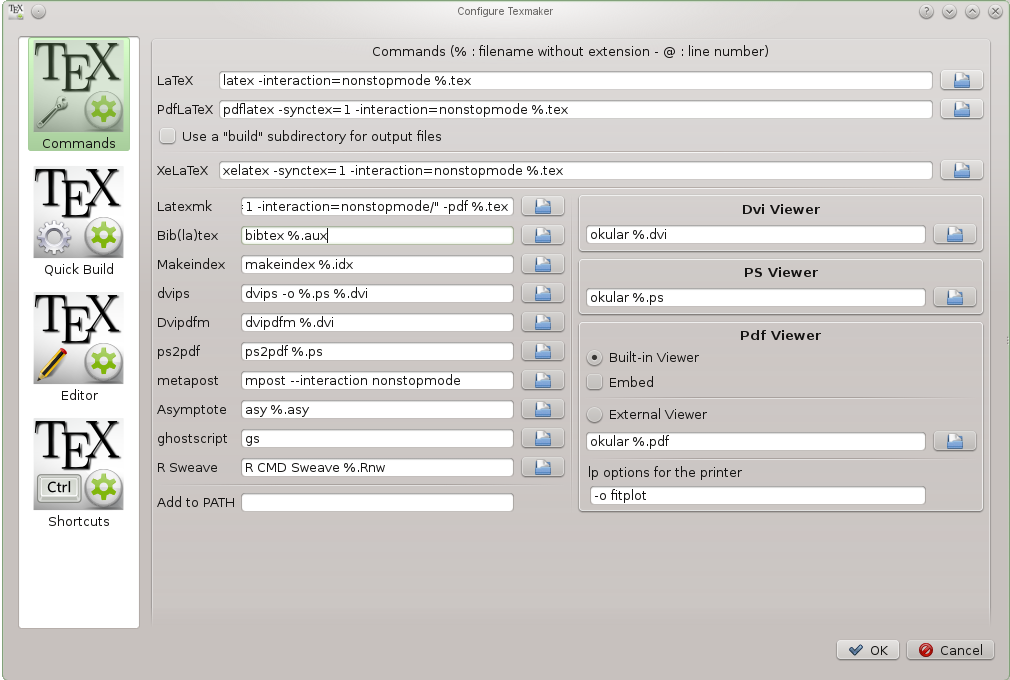
\includegraphics[width=\textwidth]{texmaker_1.png}
    \caption{Im Feld Bib(La)Tex steht normalerweise der Befehl \texttt{bibtex \%.aux}}
    \label{subfig:bibtex}
  \end{subfigure}\\[5mm]
  \begin{subfigure}{0.6\textwidth}
    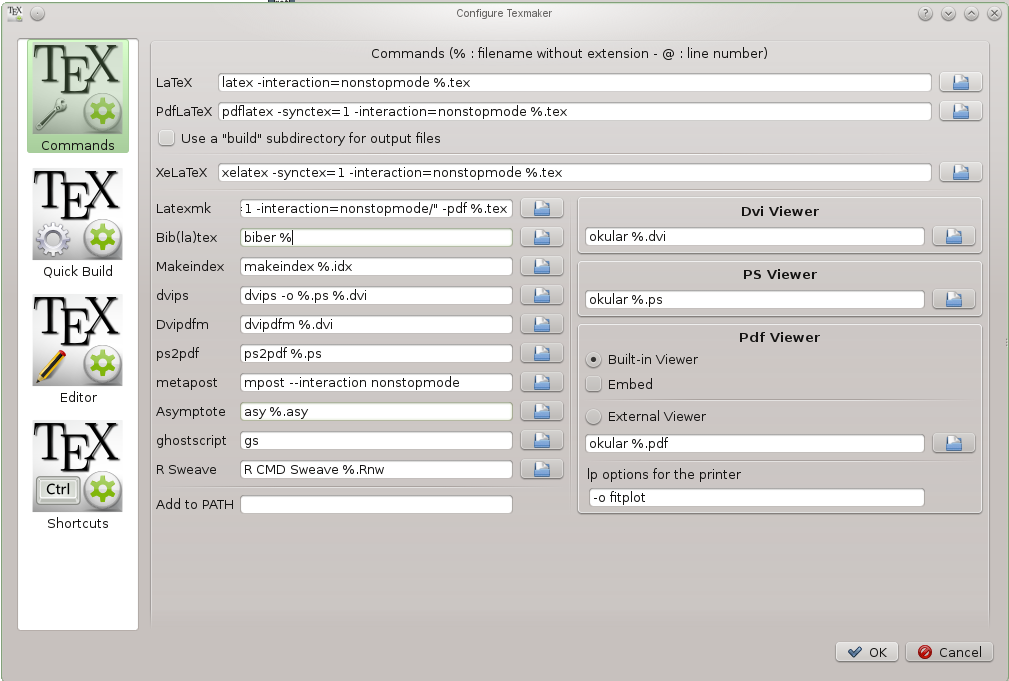
\includegraphics[width=\textwidth]{texmaker_2.png}
    \caption{Diesen Befehl sollte man auf \texttt{biber \% ändern}}
    \label{subfig:biber}
  \end{subfigure}
  \caption{Umstellen von \texttt{bibtex} zu \texttt{biber}}
\end{figure}

\begin{itemize}
  \item F1 (schnelles Übersetzen, damit eine *.bcf Datei erstellt wird)
  \item Im Dropdown-Menu zu Bibtex wechseln und mit dem Pfeil links davon biber starten. Biber verwendet dann die vorher erstellte *.bcf Datei und erzeugt eine *.bbl Datei
  \item F1 setzt nun die *.bbl Datei mit dem pdf Dokument zusammen und wenn alles funktioniert hat, sollte nun ein Literaturverzeichnis erscheinen wo im *.tex Dokument der \texttt{printbibliography} Befehl gesetzt wurde.
\end{itemize}

% subsubsection von_hand_kompilieren (end)

% subsection n_otige_schritte_zur_kompilation (end)
\newpage
\section{Tikz} % (fold)
\label{sec:tikz}

\begin{lstlisting}
\begin{figure}
\centering
  \begin{tikzpicture}[scale=0.5]
    \draw[->,thick] (-6,0) -- (6,0);
    \draw[->,thick] (0,-6) -- (0,6);
    \foreach \x in {0,1,...,10}{
      \draw[thick,blue] (\x-5,-0.1) -- (\x-5,0.1);
      \draw[thick,red] (-0.1, \x-5) -- (0.1,\x-5);
    }
    \node[below] at (6,0) {\( x \)};
    \node[left] at (0,6) { \( y \)};
  \end{tikzpicture}
\end{figure}
\end{lstlisting}

\begin{figure}[h]
\centering
  \begin{tikzpicture}[scale=0.5]
    \draw [->,thick] (-6,0) -- (6,0);
    \draw [->,thick] (0,-6) -- (0,6);
    \foreach \x in {0,1,...,10}{
      \draw[thick,blue] (\x-5,-0.1) -- (\x-5,0.1);
      \draw[thick,red] (-0.1, \x-5) -- (0.1,\x-5);
    }
    \node [below] at (6,0) {\( x \)};
    \node [left] at (0,6) { \( y \)};
  \end{tikzpicture}
\end{figure}

Mit der Tikz Umgebung kann man einfache Graphen/Zeichnungen gleich in \LaTeX\ selber setzen
\begin{itemize}
  \item \texttt{tikzpicture} ist die Umgebung, in der man Tikzbefehle verwenden kann. Diese tikzpictures kann man sehr gut in eine Gleitumgebung setzen.
  \item Kernstück von Tikz ist der \texttt{draw}-Befehl. Mit diesem Befehl werden die meisten Elemente ausgeführt.
  \item Jeder tikz-Befehl wird von einem Strichpunkt (\texttt{;}) beendet. Wird dieser vergessen, meckert Tikz \textit{Giving up on this path}
\end{itemize}
% section tikz (end)

\end{document}
